\documentclass[tikz,border=5mm]{standalone}
\usepackage{fontspec}
\setmainfont{Hiragino Sans}
\usepackage{xcolor}
\usetikzlibrary{decorations.pathreplacing}

\begin{document}
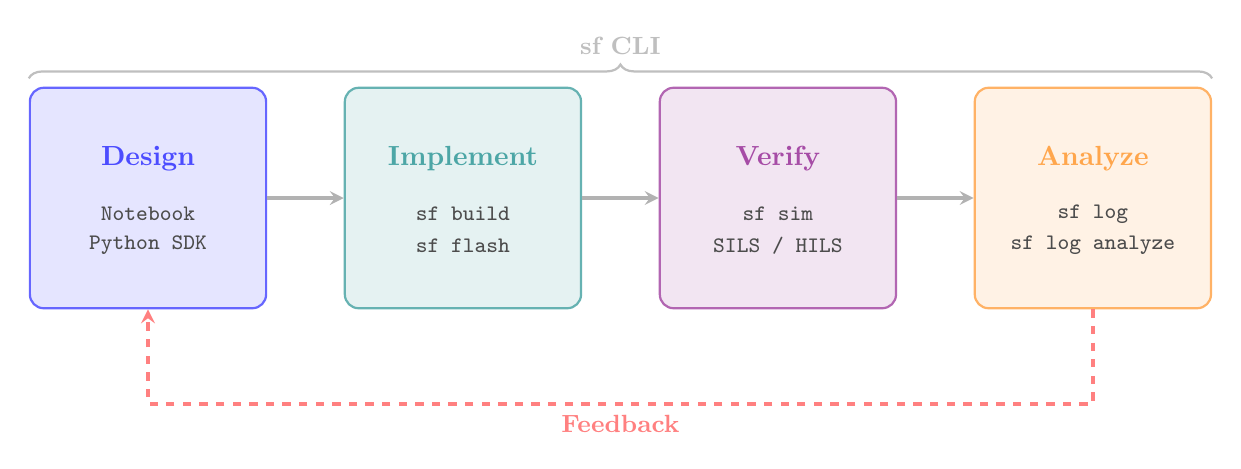
\begin{tikzpicture}[
  phase/.style={
    draw=#1!60, fill=#1!10, rounded corners=5pt,
    minimum width=30mm, minimum height=28mm,
    line width=0.8pt, align=center
  },
  ptitle/.style={
    font=\normalsize\bfseries, text=#1!70
  },
  pcmd/.style={
    font=\footnotesize\ttfamily, text=black!70
  },
  arr/.style={
    ->, thick, color=gray!60, >=stealth, line width=1.2pt
  },
  fbarr/.style={
    ->, thick, color=red!50, >=stealth, line width=1.2pt, dashed
  }
]

% Phases
\node[phase=blue] (design) at (0, 0) {};
\node[ptitle=blue] at ([yshift=5mm]design.center) {Design};
\node[pcmd] at ([yshift=-2mm]design.center) {Notebook};
\node[pcmd] at ([yshift=-6mm]design.center) {Python SDK};

\node[phase=teal] (impl) at (4, 0) {};
\node[ptitle=teal] at ([yshift=5mm]impl.center) {Implement};
\node[pcmd] at ([yshift=-2mm]impl.center) {sf build};
\node[pcmd] at ([yshift=-6mm]impl.center) {sf flash};

\node[phase=violet] (verify) at (8, 0) {};
\node[ptitle=violet] at ([yshift=5mm]verify.center) {Verify};
\node[pcmd] at ([yshift=-2mm]verify.center) {sf sim};
\node[pcmd] at ([yshift=-6mm]verify.center) {SILS / HILS};

\node[phase=orange] (analyze) at (12, 0) {};
\node[ptitle=orange] at ([yshift=5mm]analyze.center) {Analyze};
\node[pcmd] at ([yshift=-2mm]analyze.center) {sf log};
\node[pcmd] at ([yshift=-6mm]analyze.center) {sf log analyze};

% Forward arrows
\draw[arr] (design.east) -- (impl.west);
\draw[arr] (impl.east) -- (verify.west);
\draw[arr] (verify.east) -- (analyze.west);

% Feedback arrow
\draw[fbarr] (analyze.south) -- ++(0, -1.2) -| (design.south)
  node[pos=0.25, below, font=\small\bfseries, text=red!50] {Feedback};

% Top brace for sf CLI coverage
\draw[decorate, decoration={brace, amplitude=5pt, raise=3pt}, thick, gray!50]
  (design.north west) -- (analyze.north east)
  node[midway, above=8pt, font=\small\bfseries, text=gray!50] {sf CLI};

\end{tikzpicture}
\end{document}
